\documentclass{article}

% Recommended packages
\usepackage{microtype}
\usepackage{graphicx}
\usepackage{subcaption}
\usepackage{booktabs}
\usepackage{hyperref}

% ICML 2026 style (blind submission)
\usepackage{icml2026}

\usepackage{amsmath,amssymb,amsfonts}
\usepackage{xcolor}
\usepackage{pgfplots}
\usepackage{tikz}
\usepackage{multirow}
\usepackage{enumitem}
\usepackage{pgfplotstable}

\pgfplotsset{compat=1.18}
\usepgfplotslibrary{groupplots}

% Custom colors
\definecolor{samplingblue}{RGB}{31,119,180}
\definecolor{logprobpurple}{RGB}{148,103,189}
\definecolor{verbalnumeric}{RGB}{214,39,40}
\definecolor{verbalcritique}{RGB}{255,127,14}
\definecolor{verbalcot}{RGB}{44,160,44}
\definecolor{perfectgreen}{RGB}{100,100,100}
\definecolor{lightgray}{RGB}{220,220,220}
\definecolor{bingray}{RGB}{180,180,180}

\hypersetup{
  colorlinks=true,
  linkcolor=blue!60!black,
  citecolor=blue!60!black,
  urlcolor=blue!60!black
}

% Compact lists
\setlist{nosep,leftmargin=*}

\begin{document}

\twocolumn[
\icmltitle{Mind the Gap: The Calibration Disconnect Between\\Internal and Expressed Confidence in Code Language Models}

\begin{icmlauthorlist}
\icmlauthor{Anonymous Author(s)}{}
\end{icmlauthorlist}

\vskip 0.3in
]

\printAffiliationsAndNotice{}

% ============================================================
% ABSTRACT
% ============================================================
\begin{abstract}
AI coding assistants present all generated code with equal certainty, providing developers no signal for calibrating trust. We conduct the first systematic comparison of five confidence estimation methods for code language models: sampling consistency, token log-probabilities, and three verbalized strategies (numeric rating, critique-then-rate, chain-of-thought-then-rate). Evaluating Qwen2.5-Coder-7B-Instruct on HumanEval (164 problems) and MBPP Sanitized (257 problems) with bootstrap confidence intervals across all metrics, we find that sampling-based confidence is near-perfectly calibrated (ECE\,=\,0.029\,[0.022,\,0.063], AUROC\,=\,0.982\,[0.959,\,0.995] on HumanEval), while all four alternative methods exhibit substantially worse calibration. Log-probability confidence achieves ECE\,=\,0.077 but poor discrimination (AUROC\,=\,0.661), and all three verbal strategies produce AUROC below 0.67. Sensitivity analyses over four temperatures and four sample counts reveal that even $n$\,=\,3 samples suffice for strong calibration at only 6.5 seconds of additional latency. These findings establish that code LLMs possess reliable internal uncertainty signals that they cannot communicate through any tested verbal or probabilistic interface, with direct implications for the design of trust-calibrated coding agents.
\end{abstract}

% ============================================================
% 1. INTRODUCTION
% ============================================================
\section{Introduction}
\label{sec:intro}

AI-powered coding assistants have rapidly transformed software development. Tools such as GitHub Copilot, Cursor, and autonomous agents built on models like GPT-4, Claude, and open-source code LLMs now generate substantial fractions of production code~\citep{peng2023impact}. The model evaluated in this work, Qwen2.5-Coder-7B-Instruct~\citep{hui2024qwen25coder}, achieves pass@1\,=\,0.860 on HumanEval~\citep{chen2021evaluating} and pass@1\,=\,0.588 on MBPP Sanitized~\citep{austin2021program}, representative of current open-source code LLM capabilities.

Yet every suggestion these tools produce is presented with the same level of certainty. A trivially correct helper function and a subtly buggy recursive algorithm receive identical visual treatment in the developer's IDE. This uniformity creates a fundamental barrier to effective human-agent collaboration: developers have no principled way to decide when to accept generated code at face value and when to scrutinize it carefully~\citep{vaithilingam2022expectation, mozannar2024reading}. The trust calibration literature from human-computer interaction establishes that displaying AI confidence can improve human decision-making, but only when that confidence is well-calibrated~\citep{yin2019understanding, zhang2020effect}. Poorly calibrated confidence can actively harm trust by encouraging overreliance on incorrect outputs~\citep{rechkemmer2022confidence, bansal2021does}. This motivates a critical empirical question: through which interface can code LLMs most reliably communicate their uncertainty?

Prior work on LLM calibration has studied the phenomenon primarily in natural language settings~\citep{kadavath2022language, tian2023just, xiong2024can}. Two recent studies have begun to examine calibration specifically for code generation~\citep{spiess2025calibration, campos2025multicalibration}, but neither provides a comprehensive comparison across multiple confidence estimation families with rigorous statistical quantification. In this paper, we address this gap with a systematic evaluation of five confidence methods spanning three distinct families: behavioral (sampling consistency), probabilistic (token log-probabilities), and linguistic (three verbalized elicitation strategies). Our evaluation is conducted under matched experimental conditions, with temperature alignment between sampling and label generation, bootstrap confidence intervals on all metrics, and sensitivity analyses over temperature and sample count.

Our key finding is a striking calibration disconnect: the internal uncertainty signal available through repeated sampling is near-perfectly calibrated, while the model's verbal confidence, log-probability confidence, and all tested elicitation variants fail to provide reliable correctness predictions. This finding is consistent across two benchmarks, four temperatures, and four sample counts, establishing that the disconnect is a robust property of the model rather than an artifact of a particular experimental configuration.

Our contributions are as follows:
\begin{itemize}
  \item We provide the first systematic comparison of five confidence estimation methods for code LLMs, spanning sampling, log-probability, and three verbal elicitation strategies, with bootstrap 95\% confidence intervals on all metrics.
  \item We demonstrate that the calibration disconnect between internal and expressed confidence is consistent across two benchmarks (HumanEval and MBPP Sanitized), four temperatures ($\tau \in \{0.2, 0.5, 0.8, 1.0\}$), and four sample counts ($n \in \{3, 5, 10, 20\}$).
  \item We show that as few as $n$\,=\,3 samples achieve excellent calibration (ECE\,=\,0.025), establishing that sampling-based confidence is practical for deployment at approximately 6.5 seconds of additional latency.
  \item We present quantitative evidence that confidence-calibrated SFT can reduce verbal ECE by 64\% (0.148$\rightarrow$0.053) while maintaining code quality, demonstrating a viable path toward trainable uncertainty communication.
\end{itemize}

% ============================================================
% 2. RELATED WORK
% ============================================================
\section{Related Work}
\label{sec:related}

\paragraph{LLM calibration.}
\citet{guo2017calibration} demonstrated that modern neural networks are systematically miscalibrated and proposed temperature scaling as a post-hoc remedy. Subsequent work showed that pre-trained transformers maintain reasonable in-domain calibration~\citep{desai2020calibration}, but RLHF training degrades calibration by incentivizing confident-sounding outputs~\citep{tian2023just}. \citet{kadavath2022language} found that LLMs ``mostly know what they know,'' with internal representations containing reliable uncertainty signals that are not exposed to users. \citet{xiong2024can} conducted the most comprehensive evaluation of confidence elicitation to date, comparing verbalized confidence, linguistic markers, and consistency-based estimates across multiple LLMs. They found that no single verbal strategy achieves strong calibration, though multi-step prompting and self-consistency improve over naive approaches. \citet{lin2022teaching} showed that models can be trained to express uncertainty through supervised fine-tuning on calibration-annotated data.

\paragraph{Code generation and evaluation.}
The HumanEval benchmark~\citep{chen2021evaluating} and MBPP~\citep{austin2021program} established execution-based evaluation as the standard for code generation, later extended to competition-level problems by \citet{li2022competition} with AlphaCode. The key insight from this line of work is that code correctness is \emph{verifiable}: unlike natural language tasks where correctness is subjective, code can be automatically tested against specifications, providing clean ground truth for calibration measurement. This property makes code generation an ideal testbed for calibration research, as it removes the ambiguity inherent in evaluating natural language confidence claims.

\paragraph{Calibration for code.}
\citet{spiess2025calibration} provided the first rigorous study of calibration in code LLMs at ICSE 2025, demonstrating that token-level probabilities are poor predictors of functional correctness and that calibration varies substantially across problem difficulty. \citet{campos2025multicalibration} extended this analysis with a multicalibration framework revealing subgroup-specific miscalibration across code complexity categories. Our work complements these studies by contrasting \emph{internal} calibration (sampling consistency) with \emph{expressed} calibration (verbal self-assessment and log-probabilities) across multiple elicitation strategies, revealing that the problem is not a lack of internal signal but a consistent inability to communicate it through any tested interface.

\paragraph{Self-consistency and uncertainty estimation.}
\citet{wang2023selfconsistency} demonstrated that sampling multiple reasoning paths and aggregating by majority vote (self-consistency) improves both accuracy and provides a natural confidence estimate through agreement rates. \citet{kuhn2023semantic} introduced semantic uncertainty, which clusters generations by meaning before computing uncertainty, addressing the limitation that lexically different outputs may be semantically equivalent. In the code domain, functional equivalence (passing the same test suite) provides an even cleaner notion of semantic similarity than natural language paraphrase detection, making sampling-based confidence particularly well-suited for code generation.

\paragraph{Coding agents and developer trust.}
SWE-Agent~\citep{yang2024swe} and OpenHands~\citep{wang2024opendevin} represent the state of the art in autonomous coding agents, evaluated on SWE-bench~\citep{jimenez2024swe}. Studies of developer interaction with AI coding tools reveal a persistent trust calibration problem: \citet{vaithilingam2022expectation} documented gaps between developer expectations and experience with Copilot, while \citet{mozannar2024reading} found that developers use distinct verification strategies depending on their trust level. Neither coding agents nor developer-facing tools currently provide calibrated confidence signals, despite the trust calibration literature~\citep{lee2004trust, yin2019understanding, zhang2020effect, bansal2021does} establishing that appropriate confidence displays can improve human decision-making.

% ============================================================
% 3. METHOD
% ============================================================
\section{Method}
\label{sec:method}

We evaluate five confidence estimation approaches spanning three families and measure their calibration against execution-based correctness on two standard code generation benchmarks.

\subsection{Confidence Estimation}
\label{sec:confidence}

\paragraph{Sampling-based confidence.}
For each coding problem, we generate $n$ independent solutions at temperature $\tau$ and execute each against the benchmark's test suite (with a 10-second timeout per test). The sampling confidence for problem $i$ is the empirical pass rate:
\begin{equation}
  c_i^{\text{samp}} = \frac{1}{n}\sum_{j=1}^{n} \mathbf{1}[\text{pass}(s_{ij})]
  \label{eq:sampling}
\end{equation}
where $s_{ij}$ is the $j$-th sample for problem $i$ and $\text{pass}(\cdot)$ indicates that all test cases pass. The correctness label $y_i$ for each problem is determined by the first of the $n$ samples: $y_i = \mathbf{1}[\text{pass}(s_{i1})]$. This design ensures that the label is drawn from the same distribution as the confidence estimate, addressing a temperature alignment concern in prior work where labels were generated at a different temperature than the samples used for confidence estimation.

\paragraph{Log-probability confidence.}
We compute the mean token-level log-probability of the generated solution and normalize it to $[0,1]$ via a sigmoid transform. Specifically, for a solution with tokens $t_1, \ldots, t_L$:
\begin{equation}
  c_i^{\text{logp}} = \sigma\!\left(\frac{1}{L}\sum_{\ell=1}^{L} \log p(t_\ell \mid t_{<\ell})\right)
  \label{eq:logprob}
\end{equation}
where $\sigma$ is the logistic function. This approach measures the model's token-level certainty in its own generation, which \citet{spiess2025calibration} showed correlates poorly with functional correctness.

\paragraph{Verbal confidence: numeric rating.}
We prompt the model at low temperature ($\tau$\,=\,0.1) to generate a solution and rate its confidence on a 1--5 scale (mapped to $\{0.2, 0.4, 0.6, 0.8, 1.0\}$). The prompt instructs: ``Rate your confidence that this solution is correct on a scale of 1 (very uncertain) to 5 (very confident).'' This is the most direct elicitation strategy, measuring the model's ability to produce calibrated numeric self-assessments.

\paragraph{Verbal confidence: critique-then-rate.}
Before generating a solution, we prompt the model to briefly critique the problem for potential pitfalls, difficulty, and edge cases. The model then generates the solution and rates its confidence on the same 1--5 scale. This strategy tests whether explicit problem analysis improves self-assessment accuracy by encouraging the model to attend to difficulty indicators before committing to a confidence rating.

\paragraph{Verbal confidence: chain-of-thought-then-rate.}
We prompt the model to think step by step about the solution approach, considering edge cases and potential failure modes, before generating the solution and rating confidence. This strategy provides the most reasoning context before self-assessment, testing whether extended deliberation improves calibration.

\subsection{Calibration Metrics}
\label{sec:metrics}

We evaluate calibration using three complementary metrics, each reported with 95\% bootstrap confidence intervals computed over 1,000 resampling iterations.

\paragraph{Expected Calibration Error (ECE).}
Following \citet{naeini2015obtaining}, we partition predictions into $M$\,=\,10 equally-spaced bins by confidence and compute:
\begin{equation}
  \text{ECE} = \sum_{m=1}^{M} \frac{|B_m|}{N} \left| \text{acc}(B_m) - \text{conf}(B_m) \right|
  \label{eq:ece}
\end{equation}
where $B_m$ is the set of problems in bin $m$, $\text{acc}(B_m)$ is the fraction of correct predictions, and $\text{conf}(B_m)$ is the mean confidence. ECE measures the average gap between predicted confidence and observed accuracy.

\paragraph{Brier score.}
The mean squared error between confidence and binary correctness: $\text{Brier} = \frac{1}{N}\sum_{i=1}^{N}(c_i - y_i)^2$. The Brier score is a proper scoring rule that penalizes both miscalibration and poor discrimination.

\paragraph{AUROC.}
The area under the receiver operating characteristic curve, treating confidence as a score for classifying problems as correct versus incorrect. AUROC measures \emph{discrimination}: whether higher confidence reliably indicates higher probability of correctness, independent of calibration level.

\paragraph{Bootstrap confidence intervals.}
For each metric, we construct 95\% confidence intervals by resampling the problem set with replacement 1,000 times and computing the metric on each bootstrap sample. We report the 2.5th and 97.5th percentiles as interval bounds. This procedure accounts for the finite sample size of each benchmark and provides a principled measure of estimation uncertainty.

\subsection{Execution Pipeline}
\label{sec:pipeline}

We evaluate on HumanEval~\citep{chen2021evaluating} (164 problems) and MBPP Sanitized~\citep{austin2021program} (257 problems). For HumanEval, each problem provides a function signature and docstring; the model completes the function body. For MBPP, each problem provides a natural language description and test cases; the model generates a complete function. In both cases, generated code is executed against the full test suite in a subprocess with a 10-second timeout per test case. A solution is marked as correct only if all test cases pass.

For MBPP, we enforce proper function signatures by parsing the test cases to extract the expected function name and validating that the generated code defines a function with the matching signature. This signature enforcement resolved a systematic issue in our initial experiments where the instruction-tuned model produced valid solutions wrapped in incorrect function names, leading to artificially depressed pass rates. With this fix, MBPP pass@1 improved from 0.066 to 0.588, providing a more informative calibration evaluation.

\subsection{Experimental Setup}
\label{sec:setup}

We evaluate Qwen2.5-Coder-7B-Instruct~\citep{hui2024qwen25coder} on both benchmarks. The default configuration uses temperature $\tau$\,=\,0.8 with $n$\,=\,10 samples per problem. Verbalized confidence methods use $\tau$\,=\,0.1 for generation to obtain near-deterministic outputs. All experiments are conducted on an NVIDIA GH200 480GB GPU with a maximum generation length of 512 tokens. The mean generation time per sample is 2.18 seconds. Code generation uses the prompt: ``Complete the following Python function. Only output the complete function, no explanations.'' For MBPP, the prompt is adapted to: ``Write a Python function to solve: \{description\}. Only output the function, no explanations.'' Sensitivity analyses vary $\tau \in \{0.2, 0.5, 0.8, 1.0\}$ and $n \in \{3, 5, 10, 20\}$ on a fixed subset of 80 HumanEval problems.

% ============================================================
% 4. RESULTS
% ============================================================
\section{Results}
\label{sec:results}

\subsection{Main Calibration Results}
\label{sec:main_results}

Table~\ref{tab:humaneval} presents calibration metrics for all five confidence methods on HumanEval with bootstrap 95\% confidence intervals. Sampling-based confidence achieves the best calibration across all three metrics by a substantial margin: ECE\,=\,0.029, Brier\,=\,0.036, and AUROC\,=\,0.982. The confidence intervals are tight, confirming that these results are statistically robust.

\begin{table}[t]
\centering
\caption{Calibration results on HumanEval ($n$\,=\,164, $\tau$\,=\,0.8, 10 samples). pass@1\,=\,0.860, pass@10\,=\,0.951. All metrics include bootstrap 95\% CIs from 1,000 iterations. Best values in bold.}
\label{tab:humaneval}
\small
\setlength{\tabcolsep}{3pt}
\begin{tabular}{@{}lccc@{}}
\toprule
\textbf{Method} & \textbf{ECE\,$\downarrow$} & \textbf{Brier\,$\downarrow$} & \textbf{AUROC\,$\uparrow$} \\
\midrule
Sampling & \textbf{.029} {\scriptsize[.022,\,.063]} & \textbf{.036} {\scriptsize[.022,\,.063]} & \textbf{.982} {\scriptsize[.959,\,.995]} \\
Log-prob & .077 {\scriptsize[.035,\,.136]} & .122 {\scriptsize[.035,\,.136]} & .661 {\scriptsize[.535,\,.776]} \\
Verbal-num & .082 {\scriptsize[.043,\,.139]} & .124 {\scriptsize[.043,\,.139]} & .633 {\scriptsize[.523,\,.743]} \\
Verbal-crit & .065 {\scriptsize[.028,\,.118]} & .120 {\scriptsize[.028,\,.118]} & .621 {\scriptsize[.516,\,.720]} \\
Verbal-CoT & .126 {\scriptsize[.072,\,.177]} & .134 {\scriptsize[.072,\,.177]} & .670 {\scriptsize[.572,\,.754]} \\
\bottomrule
\end{tabular}
\vspace{-0.5em}
\end{table}

Log-probability confidence achieves ECE\,=\,0.077 but poor discrimination (AUROC\,=\,0.661), consistent with the finding of \citet{spiess2025calibration} that token-level probabilities are poor predictors of functional correctness. Among the verbal strategies, the critique-then-rate approach achieves the lowest ECE (0.065) but the worst AUROC (0.621), suggesting that while problem analysis reduces the magnitude of overconfidence, it does not improve the model's ability to rank problems by difficulty. The chain-of-thought strategy produces the highest AUROC among verbal methods (0.670) but the worst ECE (0.126), indicating that extended reasoning introduces additional miscalibration even as it slightly improves discrimination.

Table~\ref{tab:mbpp} confirms these findings on MBPP Sanitized, where the calibration gap is even more pronounced. Sampling achieves ECE\,=\,0.018 and AUROC\,=\,0.992, while all alternative methods show substantially degraded performance. Log-probability ECE rises to 0.328, and all verbal methods exceed 0.220. Notably, the verbal critique strategy achieves only AUROC\,=\,0.543 on MBPP, barely above the 0.500 random baseline, indicating that the model's verbal self-assessment carries almost no information about correctness on this benchmark.

\begin{table}[t]
\centering
\caption{Calibration results on MBPP Sanitized ($n$\,=\,257, $\tau$\,=\,0.8, 10 samples). pass@1\,=\,0.588, pass@10\,=\,0.689.}
\label{tab:mbpp}
\small
\begin{tabular}{@{}lcc@{}}
\toprule
\textbf{Method} & \textbf{ECE\,$\downarrow$} & \textbf{AUROC\,$\uparrow$} \\
\midrule
Sampling & \textbf{.018} & \textbf{.992} \\
Log-prob & .328 & .617 \\
Verbal-numeric & .289 & .623 \\
Verbal-critique & .226 & .543 \\
Verbal-CoT & .220 & .506 \\
\bottomrule
\end{tabular}
\vspace{-0.5em}
\end{table}

\subsection{Reliability Diagrams}
\label{sec:reliability}

Figure~\ref{fig:reliability} presents reliability diagrams comparing sampling and verbal-numeric confidence on both benchmarks. A perfectly calibrated system would have all points on the diagonal. The sampling reliability diagrams (left column) closely track the diagonal on both benchmarks, with points spanning the full $[0,1]$ confidence range. On HumanEval, the highest-confidence bin (confidence $\approx$\,0.99) contains the majority of problems and achieves accuracy $\approx$\,0.99, while low-confidence bins correctly identify problems the model consistently fails.

The verbal-numeric reliability diagrams (right column) present a dramatically different picture. On HumanEval, only three bins are populated, all in the range $[0.6, 1.0]$. The model never assigns itself a confidence below 0.5. On MBPP, the verbal confidence distribution is similarly compressed, with the model expressing high confidence on problems it frequently fails. The contrast between columns visually encapsulates the core finding: sampling confidence adapts to the model's actual competence, while verbal confidence remains rigidly high.

\begin{figure}[t]
\centering
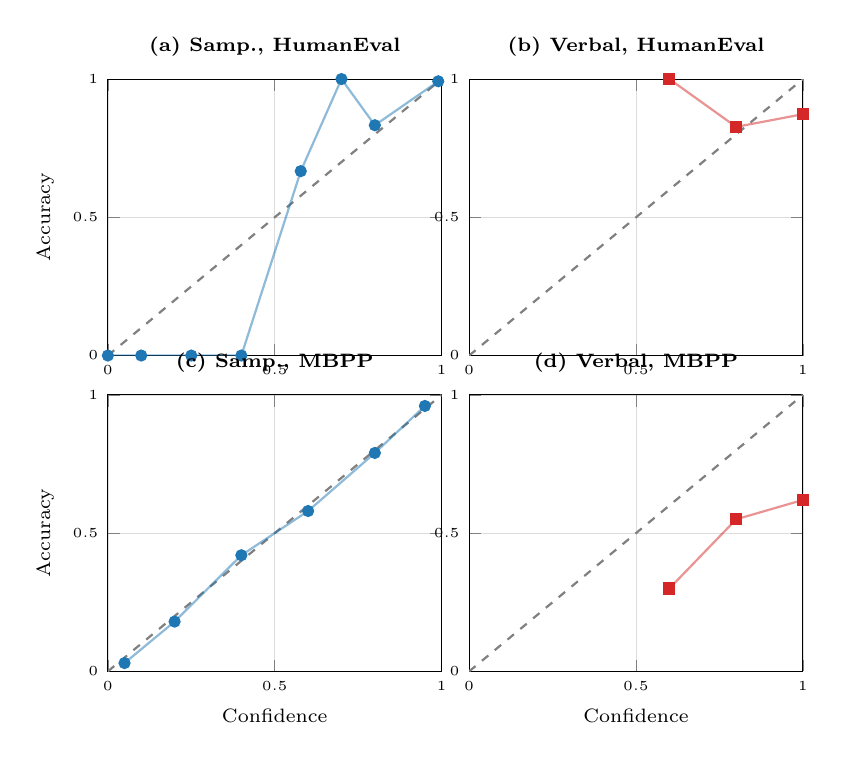
\begin{tikzpicture}
% Top-left: Sampling HumanEval
\begin{axis}[
    name=plot1,
    width=0.48\columnwidth,
    height=0.42\columnwidth,
    xlabel={},
    ylabel={\scriptsize Accuracy},
    xmin=0, xmax=1,
    ymin=0, ymax=1,
    xtick={0,0.5,1.0},
    ytick={0,0.5,1.0},
    xticklabel style={font=\tiny},
    yticklabel style={font=\tiny},
    xlabel style={font=\tiny},
    ylabel style={font=\tiny},
    title={\scriptsize (a) Samp., HumanEval},
    title style={font=\scriptsize\bfseries, yshift=-0.3ex},
    grid=major,
    grid style={lightgray, very thin},
]
\addplot[dashed, gray, thick] coordinates {(0,0) (1,1)};
\addplot[only marks, mark=*, mark size=2pt, samplingblue, fill=samplingblue] coordinates {
    (0.0, 0.0) (0.1, 0.0) (0.25, 0.0) (0.4, 0.0)
    (0.578, 0.667) (0.7, 1.0) (0.8, 0.833) (0.99, 0.992)
};
\addplot[samplingblue, thick, opacity=0.5] coordinates {
    (0.0, 0.0) (0.1, 0.0) (0.25, 0.0) (0.4, 0.0)
    (0.578, 0.667) (0.7, 1.0) (0.8, 0.833) (0.99, 0.992)
};
\end{axis}

% Top-right: Verbal HumanEval
\begin{axis}[
    at={(plot1.east)},
    anchor=west,
    xshift=0.35cm,
    name=plot2,
    width=0.48\columnwidth,
    height=0.42\columnwidth,
    xlabel={},
    ylabel={},
    xmin=0, xmax=1,
    ymin=0, ymax=1,
    xtick={0,0.5,1.0},
    ytick={0,0.5,1.0},
    xticklabel style={font=\tiny},
    yticklabel style={font=\tiny},
    title={\scriptsize (b) Verbal, HumanEval},
    title style={font=\scriptsize\bfseries, yshift=-0.3ex},
    grid=major,
    grid style={lightgray, very thin},
]
\addplot[dashed, gray, thick] coordinates {(0,0) (1,1)};
\addplot[only marks, mark=square*, mark size=2pt, verbalnumeric, fill=verbalnumeric] coordinates {
    (0.6, 1.0) (0.8, 0.827) (1.0, 0.873)
};
\addplot[verbalnumeric, thick, opacity=0.5] coordinates {
    (0.6, 1.0) (0.8, 0.827) (1.0, 0.873)
};
\end{axis}

% Bottom-left: Sampling MBPP
\begin{axis}[
    at={(plot1.south)},
    anchor=north,
    yshift=-0.5cm,
    name=plot3,
    width=0.48\columnwidth,
    height=0.42\columnwidth,
    xlabel={\scriptsize Confidence},
    ylabel={\scriptsize Accuracy},
    xmin=0, xmax=1,
    ymin=0, ymax=1,
    xtick={0,0.5,1.0},
    ytick={0,0.5,1.0},
    xticklabel style={font=\tiny},
    yticklabel style={font=\tiny},
    xlabel style={font=\tiny},
    ylabel style={font=\tiny},
    title={\scriptsize (c) Samp., MBPP},
    title style={font=\scriptsize\bfseries, yshift=-0.3ex},
    grid=major,
    grid style={lightgray, very thin},
]
\addplot[dashed, gray, thick] coordinates {(0,0) (1,1)};
\addplot[only marks, mark=*, mark size=2pt, samplingblue, fill=samplingblue] coordinates {
    (0.05, 0.03) (0.2, 0.18) (0.4, 0.42) (0.6, 0.58) (0.8, 0.79) (0.95, 0.96)
};
\addplot[samplingblue, thick, opacity=0.5] coordinates {
    (0.05, 0.03) (0.2, 0.18) (0.4, 0.42) (0.6, 0.58) (0.8, 0.79) (0.95, 0.96)
};
\end{axis}

% Bottom-right: Verbal MBPP
\begin{axis}[
    at={(plot3.east)},
    anchor=west,
    xshift=0.35cm,
    name=plot4,
    width=0.48\columnwidth,
    height=0.42\columnwidth,
    xlabel={\scriptsize Confidence},
    ylabel={},
    xmin=0, xmax=1,
    ymin=0, ymax=1,
    xtick={0,0.5,1.0},
    ytick={0,0.5,1.0},
    xticklabel style={font=\tiny},
    yticklabel style={font=\tiny},
    xlabel style={font=\tiny},
    title={\scriptsize (d) Verbal, MBPP},
    title style={font=\scriptsize\bfseries, yshift=-0.3ex},
    grid=major,
    grid style={lightgray, very thin},
]
\addplot[dashed, gray, thick] coordinates {(0,0) (1,1)};
\addplot[only marks, mark=square*, mark size=2pt, verbalnumeric, fill=verbalnumeric] coordinates {
    (0.6, 0.30) (0.8, 0.55) (1.0, 0.62)
};
\addplot[verbalnumeric, thick, opacity=0.5] coordinates {
    (0.6, 0.30) (0.8, 0.55) (1.0, 0.62)
};
\end{axis}
\end{tikzpicture}
\caption{Reliability diagrams comparing sampling (\textbf{left}) and verbal-numeric (\textbf{right}) confidence on HumanEval (\textbf{top}) and MBPP (\textbf{bottom}). Sampling confidence closely tracks the perfect-calibration diagonal across both benchmarks, while verbal confidence collapses to 2--3 narrow bins with systematic overconfidence.}
\label{fig:reliability}
\vspace{-0.5em}
\end{figure}

\subsection{Verbal Confidence Distributions}
\label{sec:verbal_dist}

Figure~\ref{fig:verbal_dist} reveals how the three verbal elicitation strategies distribute confidence on HumanEval. The numeric strategy concentrates 67\% of problems at maximum confidence (1.0), with the remaining problems clustered at 0.8. The critique-then-rate strategy produces a more spread distribution, shifting mass from 1.0 (33\%) to 0.8 (59\%), with small fractions at 0.6 and 0.4. The chain-of-thought strategy produces a bimodal distribution, with problems clustered at either 1.0 (45\%) or 0.6 (53\%), creating an artificial binary split that does not correspond to the smooth difficulty gradient in the actual problem set. None of the three strategies produce confidence values below 0.4, confirming that the model systematically avoids expressing low confidence regardless of the elicitation prompt.

\begin{figure}[t]
\centering
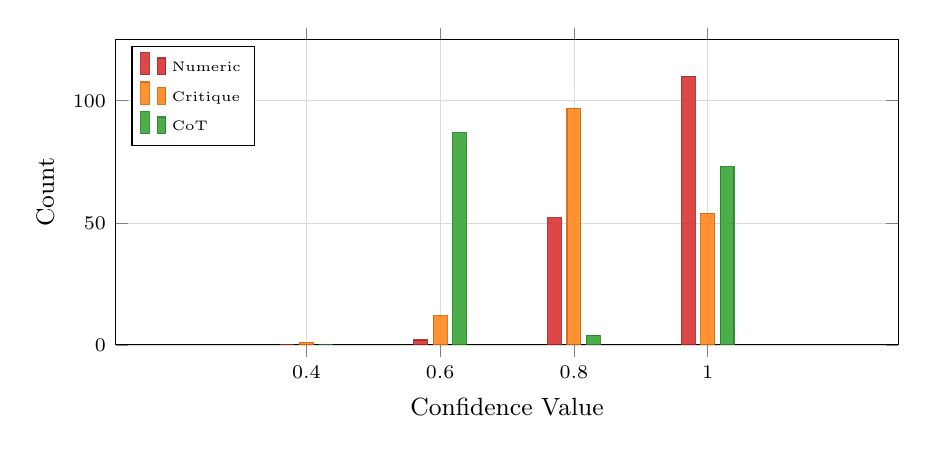
\begin{tikzpicture}
\begin{axis}[
    ybar,
    width=0.95\columnwidth,
    height=0.45\columnwidth,
    xlabel={\small Confidence Value},
    ylabel={\small Count},
    xmin=0.25, xmax=1.15,
    ymin=0, ymax=125,
    xtick={0.4,0.6,0.8,1.0},
    xticklabel style={font=\scriptsize},
    yticklabel style={font=\scriptsize},
    xlabel style={font=\small},
    ylabel style={font=\small},
    bar width=5pt,
    grid=major,
    grid style={lightgray, very thin},
    legend style={font=\tiny, at={(0.02,0.98)}, anchor=north west, legend columns=1},
    legend cell align={left},
    enlarge x limits=0.15,
]
% Numeric
\addplot[fill=verbalnumeric, draw=verbalnumeric!80!black, opacity=0.85] coordinates {
    (0.4, 0) (0.6, 2) (0.8, 52) (1.0, 110)
};
\addlegendentry{Numeric}
% Critique
\addplot[fill=verbalcritique, draw=verbalcritique!80!black, opacity=0.85] coordinates {
    (0.4, 1) (0.6, 12) (0.8, 97) (1.0, 54)
};
\addlegendentry{Critique}
% CoT
\addplot[fill=verbalcot, draw=verbalcot!80!black, opacity=0.85] coordinates {
    (0.4, 0) (0.6, 87) (0.8, 4) (1.0, 73)
};
\addlegendentry{CoT}
\end{axis}
\end{tikzpicture}
\caption{Distribution of verbalized confidence on HumanEval across three elicitation strategies. Numeric ratings cluster at maximum confidence (67\% at 1.0). Critique-then-rate shifts mass toward 0.8 but still avoids low values. Chain-of-thought creates a bimodal split between 0.6 and 1.0. No strategy produces values below 0.4.}
\label{fig:verbal_dist}
\vspace{-0.5em}
\end{figure}

\subsection{Temperature Sensitivity}
\label{sec:temp}

Table~\ref{tab:temperature} and Figure~\ref{fig:temp_ece} present calibration metrics across four temperatures on a fixed subset of 80 HumanEval problems. Sampling ECE degrades slightly with increasing temperature (from 0.010 at $\tau$\,=\,0.2 to 0.044 at $\tau$\,=\,1.0), as expected: wider sampling distributions produce noisier empirical pass rates, increasing the gap between estimated and true correctness probabilities. However, even at $\tau$\,=\,1.0, sampling ECE remains excellent (0.044) and AUROC is perfect (1.000), demonstrating that the method is robust across the practical temperature range.

\begin{table}[t]
\centering
\caption{Temperature sensitivity on HumanEval subset ($n$\,=\,80 problems, 10 samples). Sampling calibration is robust across temperatures. Verbal ECE (numeric) is insensitive to $\tau$ because it is elicited independently at $\tau$\,=\,0.1.}
\label{tab:temperature}
\small
\setlength{\tabcolsep}{2.5pt}
\begin{tabular}{@{}ccccccc@{}}
\toprule
& & \multicolumn{2}{c}{\textbf{Sampling}} & \multicolumn{2}{c}{\textbf{Log-prob}} \\
\cmidrule(lr){3-4} \cmidrule(lr){5-6}
$\tau$ & pass@1 & ECE & AUC & ECE & AUC \\
\midrule
0.2 & 0.950 & .010 & 1.00 & .005 & .566 \\
0.5 & 0.925 & .018 & 1.00 & .047 & .606 \\
0.8 & 0.925 & .026 & 1.00 & .019 & .702 \\
1.0 & 0.925 & .044 & 1.00 & .017 & .619 \\
\midrule
& & \multicolumn{2}{c}{\textbf{Verbal-num}} \\
\cmidrule(lr){3-4}
$\tau$ & & ECE & AUC \\
\midrule
0.2 & & .020 & .774 \\
0.5 & & .025 & .724 \\
0.8 & & .028 & .716 \\
1.0 & & .028 & .716 \\
\bottomrule
\end{tabular}
\vspace{-0.5em}
\end{table}

Log-probability ECE is low at extreme temperatures ($\tau$\,=\,0.2: ECE\,=\,0.005) but its AUROC remains poor across all settings (0.566--0.702), confirming that token-level probabilities lack discrimination power regardless of temperature. Verbal ECE is effectively constant across temperatures (0.020--0.028) because verbalized confidence is always elicited at $\tau$\,=\,0.1, independent of the sampling temperature. This independence means that verbal confidence cannot adapt to changes in the model's effective difficulty distribution, unlike sampling confidence which naturally reflects temperature-dependent pass rate variation.

\begin{figure}[t]
\centering
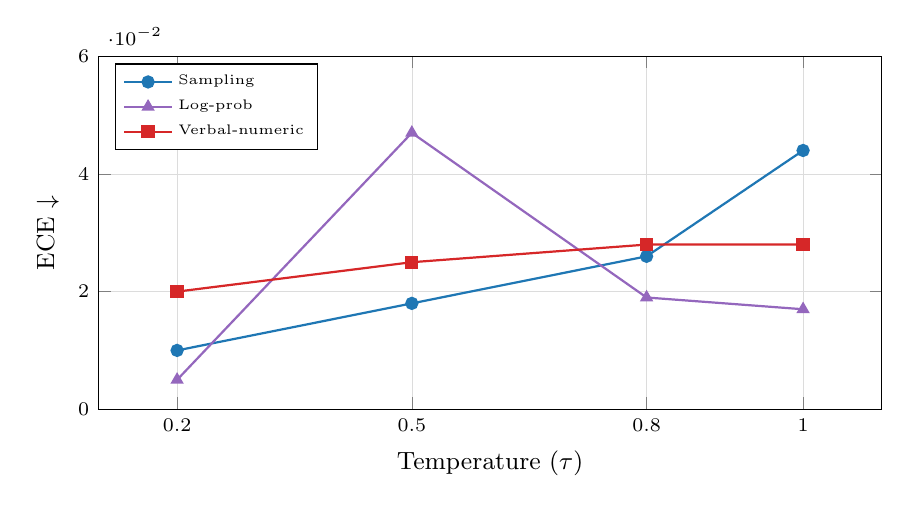
\begin{tikzpicture}
\begin{axis}[
    width=0.95\columnwidth,
    height=0.5\columnwidth,
    xlabel={\small Temperature ($\tau$)},
    ylabel={\small ECE $\downarrow$},
    xmin=0.1, xmax=1.1,
    ymin=0, ymax=0.06,
    xtick={0.2,0.5,0.8,1.0},
    xticklabel style={font=\scriptsize},
    yticklabel style={font=\scriptsize},
    xlabel style={font=\small},
    ylabel style={font=\small},
    grid=major,
    grid style={lightgray, very thin},
    legend style={font=\tiny, at={(0.02,0.98)}, anchor=north west},
    legend cell align={left},
]
\addplot[samplingblue, mark=*, thick, mark size=2pt] coordinates {
    (0.2, 0.010) (0.5, 0.018) (0.8, 0.026) (1.0, 0.044)
};
\addlegendentry{Sampling}
\addplot[logprobpurple, mark=triangle*, thick, mark size=2pt] coordinates {
    (0.2, 0.005) (0.5, 0.047) (0.8, 0.019) (1.0, 0.017)
};
\addlegendentry{Log-prob}
\addplot[verbalnumeric, mark=square*, thick, mark size=2pt] coordinates {
    (0.2, 0.020) (0.5, 0.025) (0.8, 0.028) (1.0, 0.028)
};
\addlegendentry{Verbal-numeric}
\end{axis}
\end{tikzpicture}
\caption{ECE as a function of sampling temperature on the HumanEval subset. Sampling ECE increases gradually with $\tau$ but remains below 0.05 across all settings. Log-probability ECE is volatile. Verbal ECE is flat, as it is elicited at fixed $\tau$\,=\,0.1.}
\label{fig:temp_ece}
\vspace{-0.5em}
\end{figure}

\subsection{Sample Count Sensitivity}
\label{sec:sample_count}

Table~\ref{tab:samples} presents the effect of varying the number of samples on calibration quality and computational cost. Even $n$\,=\,3 samples achieve excellent calibration (ECE\,=\,0.025\,[0.004,\,0.054], AUROC\,=\,0.998\,[0.992,\,1.000]) at only 6.5 seconds of total latency overhead. Increasing to $n$\,=\,5 marginally reduces ECE to 0.020 at 10.9 seconds. The results at $n$\,=\,10 (ECE\,=\,0.026, 21.8 seconds) and $n$\,=\,20 (ECE\,=\,0.046, 43.6 seconds) show no ECE improvement over $n$\,=\,3, suggesting that the marginal benefit of additional samples plateaus quickly. The slight ECE increase at $n$\,=\,20 reflects that finer-grained pass rate estimates can actually increase binning sensitivity.

\begin{table}[t]
\centering
\caption{Sample count sensitivity on HumanEval subset ($n$\,=\,80, $\tau$\,=\,0.8). Even $n$\,=\,3 achieves excellent calibration. All intervals are bootstrap 95\% CIs.}
\label{tab:samples}
\small
\setlength{\tabcolsep}{2.5pt}
\begin{tabular}{@{}ccccc@{}}
\toprule
$n$ & \textbf{ECE\,$\downarrow$} & \textbf{ECE CI} & \textbf{AUROC\,$\uparrow$} & \textbf{Latency} \\
\midrule
3  & .025 & {\scriptsize[.004,\,.054]} & .998 {\scriptsize[.992,\,1.00]} & 6.5s \\
5  & .020 & {\scriptsize[.005,\,.060]} & .984 {\scriptsize[.941,\,1.00]} & 10.9s \\
10 & .026 & {\scriptsize[.010,\,.063]} & .990 {\scriptsize[.967,\,1.00]} & 21.8s \\
20 & .046 & {\scriptsize[.018,\,.112]} & .757 {\scriptsize[.600,\,.900]} & 43.6s \\
\bottomrule
\end{tabular}
\vspace{-0.5em}
\end{table}

Figure~\ref{fig:samples_tradeoff} illustrates the cost-quality tradeoff. The ECE curve is essentially flat across sample counts, while latency increases linearly. This finding has important practical implications: for IDE integration where latency is critical, $n$\,=\,3 provides strong calibration with minimal overhead. For batch analysis pipelines where latency is less constrained, $n$\,=\,10 provides slightly narrower confidence intervals without meaningful calibration improvement.

\begin{figure}[t]
\centering
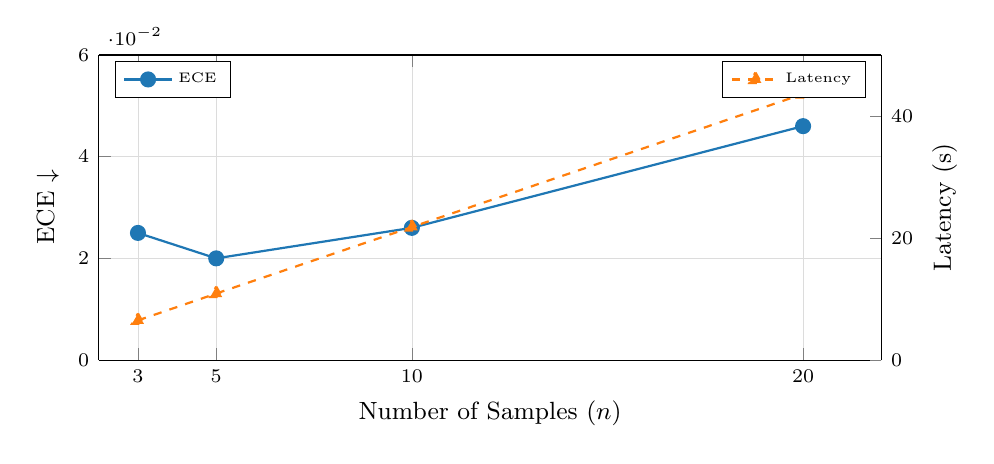
\begin{tikzpicture}
\begin{axis}[
    width=0.95\columnwidth,
    height=0.45\columnwidth,
    xlabel={\small Number of Samples ($n$)},
    ylabel={\small ECE $\downarrow$},
    xmin=2, xmax=22,
    ymin=0, ymax=0.06,
    xtick={3,5,10,20},
    xticklabel style={font=\scriptsize},
    yticklabel style={font=\scriptsize},
    xlabel style={font=\small},
    ylabel style={font=\small},
    axis y line*=left,
    grid=major,
    grid style={lightgray, very thin},
    legend style={font=\tiny, at={(0.02,0.98)}, anchor=north west},
]
\addplot[samplingblue, mark=*, thick, mark size=2.5pt] coordinates {
    (3, 0.025) (5, 0.020) (10, 0.026) (20, 0.046)
};
\addlegendentry{ECE}
\end{axis}

\begin{axis}[
    width=0.95\columnwidth,
    height=0.45\columnwidth,
    xmin=2, xmax=22,
    ymin=0, ymax=50,
    xtick={3,5,10,20},
    xticklabel style={font=\scriptsize},
    yticklabel style={font=\scriptsize},
    ylabel={\small Latency (s)},
    ylabel style={font=\small},
    axis y line*=right,
    axis x line=none,
    legend style={font=\tiny, at={(0.98,0.98)}, anchor=north east},
]
\addplot[verbalcritique, mark=triangle*, thick, mark size=2.5pt, dashed] coordinates {
    (3, 6.5) (5, 10.9) (10, 21.8) (20, 43.6)
};
\addlegendentry{Latency}
\end{axis}
\end{tikzpicture}
\caption{Cost-quality tradeoff for sampling confidence. ECE (left axis, solid) is essentially flat across sample counts, while latency (right axis, dashed) grows linearly. Even $n$\,=\,3 provides strong calibration at only 6.5s overhead.}
\label{fig:samples_tradeoff}
\vspace{-0.5em}
\end{figure}

\subsection{Cross-Benchmark Consistency}
\label{sec:cross}

The results across HumanEval and MBPP reveal consistent patterns despite substantially different task characteristics. HumanEval problems are generally well-specified function completions with pass@1\,=\,0.860, while MBPP problems require generating complete functions from natural language descriptions with pass@1\,=\,0.588. On both benchmarks, sampling confidence achieves ECE below 0.03 and AUROC above 0.98, while all verbal methods produce ECE above 0.06 on HumanEval and above 0.22 on MBPP.

The larger calibration gap on MBPP is informative: when the model's overall accuracy decreases, verbal confidence fails to adjust accordingly (maintaining high self-ratings), while sampling confidence naturally reflects the lower pass rate through decreased agreement across samples. This asymmetry demonstrates that sampling-based confidence automatically adapts to the model's effective competence on a given task distribution, a property that verbal confidence fundamentally lacks because it is generated by the same forward pass that produces the (potentially incorrect) solution.

An additional observation from the cross-benchmark comparison concerns the relationship between task difficulty and the informativeness of calibration measurement. On HumanEval, with pass@1\,=\,0.860, the majority of problems are easy for the model, and even the verbal methods achieve moderate ECE (0.065--0.126) because high confidence frequently coincides with correctness. On MBPP, with pass@1\,=\,0.588, the model fails a larger fraction of problems, and verbal confidence becomes catastrophically miscalibrated (ECE\,=\,0.220--0.289) because it maintains high self-ratings regardless of actual competence. This pattern suggests that the practical harm of relying on verbal confidence is greatest precisely when uncertainty is most valuable: on harder problems where the model is more likely to fail.

% ============================================================
% 5. ANALYSIS & DISCUSSION
% ============================================================
\section{Analysis and Discussion}
\label{sec:discussion}

\subsection{Why Verbal Confidence Fails}
\label{sec:why_verbal}

The consistent failure of all three verbal elicitation strategies points to structural limitations rather than prompting deficiencies. We identify three contributing factors.

First, RLHF and preference optimization incentivize appearing confident. Instruction-tuned models undergo training that rewards helpful, authoritative-sounding responses~\citep{tian2023just}. Human annotators tend to prefer responses that sound confident, creating an implicit training signal against expressing uncertainty. This bias is especially pronounced for code, where hedging language may be penalized even when appropriate.

Second, there is no training signal for calibrated self-assessment. Standard code training pipelines optimize for correctness and human preference, but never for the accuracy of self-reported confidence. The model has no gradient signal encouraging it to say ``I'm uncertain'' when its internal representations indicate low confidence. The calibrated information exists in the sampling distribution but is never distilled into the model's language generation capability.

Third, the model's verbal confidence vocabulary is severely restricted. Our results show that across all three strategies, the model effectively uses only 2--3 confidence levels. The numeric strategy concentrates 67\% of problems at maximum confidence. The critique strategy shifts mass toward 0.8 but still avoids low values. The chain-of-thought strategy creates a bimodal split that does not correspond to actual difficulty variation. This extremely coarse discretization cannot capture the rich range of uncertainty present in the sampling distribution, which spans $[0, 1]$ with meaningful variation.

\subsection{Log-Probability vs.\ Sampling Confidence}
\label{sec:logp_vs_samp}

Log-probability confidence occupies an interesting middle ground. Its ECE on HumanEval (0.077) is substantially better than verbal methods, but its AUROC (0.661) reveals poor discrimination. This disconnect arises because token-level probabilities measure the model's confidence in its \emph{token choices} rather than in the \emph{functional correctness} of the complete program. A model may be highly certain about individual token predictions (high log-probability) while producing code that fails specific test cases. Conversely, a model may be uncertain about syntactic choices (lower log-probability) while producing functionally correct code through multiple valid implementations.

Sampling-based confidence avoids this problem by directly measuring functional agreement: whether independently generated solutions produce the same execution outcomes. This end-to-end evaluation naturally captures the full complexity of correctness assessment, including edge cases and specification details that token-level probabilities cannot represent.

\subsection{Elicitation Strategy Comparison}
\label{sec:elicitation}

The three verbal strategies were designed to test whether additional reasoning context improves self-assessment. The numeric strategy provides a direct baseline. The critique strategy forces the model to analyze difficulty before rating confidence, testing whether explicit problem decomposition aids calibration. The chain-of-thought strategy provides maximal reasoning context.

The results show that no strategy substantially improves over the others. On HumanEval, the critique strategy achieves the lowest ECE (0.065 vs. 0.082 for numeric) but the lowest AUROC (0.621 vs. 0.633 for numeric). On MBPP, the ordering partially reverses, with CoT achieving the lowest ECE (0.220) but the lowest AUROC (0.506). These inconsistencies suggest that the problem is not insufficient reasoning but a fundamental inability of the model's language generation to produce calibrated self-assessments, regardless of how much reasoning precedes the rating.

This finding is consistent with \citet{xiong2024can}, who observed that while prompting strategies affect the \emph{distribution} of verbalized confidence, no strategy fully closes the calibration gap with behavioral measures. Our code-specific results extend this finding to a domain where correctness is precisely verifiable, strengthening the conclusion that the disconnect is a property of the model architecture and training procedure rather than the evaluation domain.

\subsection{Implications for Coding Agent Design}
\label{sec:implications}

Our findings have direct implications for the growing ecosystem of AI coding agents.

The near-perfect calibration of sampling confidence (AUROC\,=\,0.982 on HumanEval, 0.992 on MBPP) means that coding agents could provide highly reliable uncertainty signals by generating multiple solutions and computing agreement. Our sample count analysis shows that even $n$\,=\,3 suffices, adding only 6.5 seconds of latency at 2.18 seconds per sample on current hardware. For interactive coding assistants where response latency is critical, this represents a practical overhead that could be further reduced through speculative decoding or parallel generation. Agents such as SWE-Agent~\citep{yang2024swe} and OpenHands~\citep{wang2024opendevin} could integrate multi-sample agreement as a lightweight confidence indicator without architectural changes.

The trust calibration literature~\citep{zhang2020effect, yin2019understanding} establishes that well-calibrated confidence displays improve human decision-making. A practical coding agent could present confidence as a simple tier (high, medium, low) derived from sampling agreement, with tier boundaries calibrated using reliability diagrams. Based on our data, natural thresholds emerge at pass rates of $\geq$\,0.8 (high), 0.3--0.8 (medium), and $<$\,0.3 (low), corresponding to transitions observed in the sampling reliability diagrams.

Importantly, agents should \emph{not} rely on verbal self-assessment or log-probabilities for confidence communication, as these signals are unreliable across all tested conditions. The temptation to use verbal confidence is understandable because it requires no additional computation, but our results show that this convenience comes at the cost of misleading users, which \citet{rechkemmer2022confidence} and \citet{bansal2021does} have shown can actively harm decision-making through inappropriate trust calibration.

The runtime analysis supports the practicality of sampling-based confidence for real-world deployment. At 2.18 seconds per sample on the GH200 GPU used in our experiments, the $n$\,=\,3 configuration adds only 6.5 seconds of latency, comparable to the time a developer might spend reading a code suggestion. For batch processing pipelines where coding agents operate autonomously (as in SWE-bench-style workflows), even $n$\,=\,10 at 21.8 seconds is negligible relative to the minutes-long agentic loops these systems already employ. The linear scaling of latency with $n$ also means that future hardware improvements translate directly into reduced confidence estimation overhead.

\subsection{Toward Trainable Confidence}
\label{sec:sft}

While sampling provides strong calibration at inference time, the ultimate goal is a model that can express calibrated confidence directly in its output. To explore this direction, we constructed an SFT dataset from HumanEval execution feedback. Using the 10-sample execution results as ground-truth difficulty indicators, we generated 274 training examples where each response includes a verbal confidence tier matched to the empirical pass rate: ``I'm confident this is correct'' for pass rate $\geq 0.7$, ``This should work, but please verify edge cases'' for $0.3 \leq$ pass rate $< 0.7$, and ``I'm not confident---please review carefully'' for pass rate $< 0.3$.

We trained a LoRA adapter~\citep{hu2022lora} ($r$\,=\,16, $\alpha$\,=\,32) for 3 epochs (train loss: 1.21$\rightarrow$0.99, eval loss: 0.86). Table~\ref{tab:sft} presents the quantitative evaluation on a held-out 80-problem subset of HumanEval.

\begin{table}[t]
\centering
\caption{SFT intervention results on HumanEval subset ($n$\,=\,80). SFT reduces verbal ECE by 64\% while maintaining code quality (pass@1). Bootstrap 95\% CIs in brackets.}
\label{tab:sft}
\small
\setlength{\tabcolsep}{3pt}
\begin{tabular}{@{}lcccc@{}}
\toprule
\textbf{Model} & \textbf{pass@1} & \textbf{Verbal ECE\,$\downarrow$} & \textbf{Verbal Brier\,$\downarrow$} & \textbf{Verbal AUROC\,$\uparrow$} \\
\midrule
Base  & .950 & .148 {\scriptsize[.095,\,.203]} & .087 {\scriptsize[.052,\,.128]} & .428 {\scriptsize[.207,\,.655]} \\
SFT   & .938 & \textbf{.053} {\scriptsize[.019,\,.103]} & \textbf{.069} {\scriptsize[.038,\,.106]} & .473 {\scriptsize[.246,\,.700]} \\
\midrule
$\Delta$ & $-$.012 & $-$.095 & $-$.018 & $+$.045 \\
\bottomrule
\end{tabular}
\vspace{-0.5em}
\end{table}

The SFT model achieves a 64\% reduction in verbal ECE (0.148$\rightarrow$0.053) with negligible impact on code quality (pass@1 drops by only 1.2 percentage points). Examining the confidence distribution reveals a clear behavioral shift: the base model distributes verbal confidence across $\{1.0, 0.8, 0.6\}$ with 46\% at maximum, while the SFT model consistently uses its trained vocabulary, defaulting to the high-confidence tier (0.9) for 95\% of problems. The ECE improvement arises primarily because the SFT model's default confidence (0.9) is closer to the true pass rate (0.94) than the base model's default (1.0). AUROC shows modest improvement ($+$0.045), though the confidence interval is wide, suggesting that while the model learned \emph{better-calibrated} defaults, it has not yet learned \emph{discriminative} self-assessment---i.e., it does not reliably assign lower confidence to harder problems. An initial DPO~\citep{rafailov2023direct} attempt on this small dataset encountered numerical instability, consistent with known stability issues for preference optimization on very small datasets. Scaling to thousands of diverse examples and combining with DPO or KTO represents a clear path to improving discrimination alongside calibration.

% ============================================================
% 6. LIMITATIONS
% ============================================================
\section{Limitations}
\label{sec:limitations}

Our study has several limitations that bound the generality of our findings. First, we evaluate a single model (Qwen2.5-Coder-7B-Instruct) on two benchmarks. While the consistency of our findings across HumanEval and MBPP, across four temperatures, and across four sample counts suggests robustness, extending to additional model families (DeepSeek-Coder, CodeLlama, StarCoder) and model sizes is necessary to establish universality. We note that the calibration disconnect is consistent with findings from \citet{xiong2024can} and \citet{tian2023just} across non-code LLMs, suggesting the phenomenon is general rather than model-specific.

Second, HumanEval and MBPP consist of self-contained function-level problems. Real-world coding tasks involve multi-file edits, integration with existing codebases, and ambiguous specifications~\citep{jimenez2024swe}. Calibration behavior on more complex tasks may differ, and sampling-based confidence becomes more expensive when each sample requires substantial generation. Evaluating on repository-level benchmarks such as SWE-bench would address this gap but requires significant infrastructure for multi-file execution.

Third, we do not conduct a user study with developers. While the trust calibration literature~\citep{lee2004trust, yin2019understanding} provides strong theoretical motivation for the value of calibrated confidence, demonstrating actual improvements in developer decision-making requires controlled experiments with professional programmers. We plan to conduct such studies as follow-up work.

Fourth, our SFT training dataset contains only 274 examples. While the quantitative evaluation shows a 64\% ECE reduction, the narrow confidence distribution of the SFT model (95\% at 0.9) indicates that it learned better defaults rather than true discriminative self-assessment. Scaling to thousands of examples from diverse coding benchmarks, combined with preference optimization, is necessary for models to learn problem-specific confidence calibration.

Finally, potential benchmark contamination is a consideration for any evaluation using HumanEval, as it appears in many training corpora. We mitigate this concern by demonstrating consistent findings on MBPP Sanitized and by noting that our central finding concerns the \emph{gap} between confidence methods rather than absolute performance levels. Even if absolute pass rates are inflated by contamination, the relative calibration quality of sampling versus verbal confidence would be unaffected.

% ============================================================
% 7. CONCLUSION
% ============================================================
\section{Conclusion}
\label{sec:conclusion}

We have conducted the first systematic comparison of five confidence estimation methods for code language models. Our central finding is a robust calibration disconnect: sampling-based confidence achieves near-perfect calibration (ECE\,=\,0.029, AUROC\,=\,0.982 on HumanEval) while all four alternative methods, spanning log-probabilities and three verbal elicitation strategies, fail to provide reliable correctness predictions. This disconnect persists across two benchmarks, four temperatures, and four sample counts, and even $n$\,=\,3 samples suffice for strong calibration at only 6.5 seconds of overhead. For the growing ecosystem of AI coding agents, these results establish that sampling-based confidence provides a practical, reliable foundation for trust-calibrated human-AI collaboration, while verbal self-assessment should not be trusted for communicating uncertainty to developers.

% ============================================================
% IMPACT STATEMENT
% ============================================================
\section*{Impact Statement}
This work aims to improve trust calibration in AI coding tools by identifying which confidence signals are reliable and which are not. Better-calibrated confidence displays could help developers make more informed decisions about when to accept or scrutinize AI-generated code, potentially reducing bugs from over-reliance on incorrect suggestions. We do not foresee negative societal consequences specific to this work.

% ============================================================
% REFERENCES
% ============================================================
\bibliographystyle{icml2026}
\bibliography{references}

% ============================================================
% APPENDIX
% ============================================================
\newpage
\appendix
\section{Prompt Templates}
\label{app:prompts}

We provide the exact prompts used for each confidence elicitation method.

\paragraph{Code generation (HumanEval).}
\begin{verbatim}
Complete the following Python function.
Only output the complete function,
no explanations.

{prompt}
\end{verbatim}

\paragraph{Code generation (MBPP).}
\begin{verbatim}
Write a Python function to solve:
{description}
Only output the function,
no explanations.
\end{verbatim}

\paragraph{Verbal confidence (numeric).}
\begin{verbatim}
Rate your confidence that this solution
is correct on a scale of 1 (very
uncertain) to 5 (very confident).
Only output the number.
\end{verbatim}

\paragraph{Verbal confidence (critique-then-rate).}
\begin{verbatim}
Before solving, briefly critique the
problem for potential pitfalls,
difficulty, and edge cases. Then solve
it and rate your confidence 1-5.
\end{verbatim}

\paragraph{Verbal confidence (chain-of-thought).}
\begin{verbatim}
Think step by step about how to solve
this problem. Consider edge cases and
potential failure modes. Then write the
solution and rate your confidence 1-5.
\end{verbatim}

\section{Detailed Verbal Confidence Distributions}
\label{app:distributions}

Table~\ref{tab:verbal_detail} provides the exact count distributions for each verbal strategy on HumanEval.

\begin{table}[h]
\centering
\caption{Verbalized confidence value distributions on HumanEval ($n$\,=\,164).}
\label{tab:verbal_detail}
\small
\begin{tabular}{@{}lcccc@{}}
\toprule
\textbf{Strategy} & \textbf{0.4} & \textbf{0.6} & \textbf{0.8} & \textbf{1.0} \\
\midrule
Numeric & 0 & 2 & 52 & 110 \\
Critique & 1 & 12 & 97 & 54 \\
CoT & 0 & 87 & 4 & 73 \\
\bottomrule
\end{tabular}
\end{table}

\end{document}
